\documentclass[]{article}
\usepackage{lmodern}
\usepackage{amssymb,amsmath}
\usepackage{ifxetex,ifluatex}
\usepackage{fixltx2e} % provides \textsubscript
\ifnum 0\ifxetex 1\fi\ifluatex 1\fi=0 % if pdftex
  \usepackage[T1]{fontenc}
  \usepackage[utf8]{inputenc}
\else % if luatex or xelatex
  \ifxetex
    \usepackage{mathspec}
  \else
    \usepackage{fontspec}
  \fi
  \defaultfontfeatures{Ligatures=TeX,Scale=MatchLowercase}
\fi
% use upquote if available, for straight quotes in verbatim environments
\IfFileExists{upquote.sty}{\usepackage{upquote}}{}
% use microtype if available
\IfFileExists{microtype.sty}{%
\usepackage{microtype}
\UseMicrotypeSet[protrusion]{basicmath} % disable protrusion for tt fonts
}{}
\usepackage[margin=1in]{geometry}
\usepackage{hyperref}
\hypersetup{unicode=true,
            pdftitle={Criação de Gráficos em R {[}Dispersão{]}},
            pdfauthor={Amanda Coração},
            pdfborder={0 0 0},
            breaklinks=true}
\urlstyle{same}  % don't use monospace font for urls
\usepackage{color}
\usepackage{fancyvrb}
\newcommand{\VerbBar}{|}
\newcommand{\VERB}{\Verb[commandchars=\\\{\}]}
\DefineVerbatimEnvironment{Highlighting}{Verbatim}{commandchars=\\\{\}}
% Add ',fontsize=\small' for more characters per line
\usepackage{framed}
\definecolor{shadecolor}{RGB}{248,248,248}
\newenvironment{Shaded}{\begin{snugshade}}{\end{snugshade}}
\newcommand{\AlertTok}[1]{\textcolor[rgb]{0.94,0.16,0.16}{#1}}
\newcommand{\AnnotationTok}[1]{\textcolor[rgb]{0.56,0.35,0.01}{\textbf{\textit{#1}}}}
\newcommand{\AttributeTok}[1]{\textcolor[rgb]{0.77,0.63,0.00}{#1}}
\newcommand{\BaseNTok}[1]{\textcolor[rgb]{0.00,0.00,0.81}{#1}}
\newcommand{\BuiltInTok}[1]{#1}
\newcommand{\CharTok}[1]{\textcolor[rgb]{0.31,0.60,0.02}{#1}}
\newcommand{\CommentTok}[1]{\textcolor[rgb]{0.56,0.35,0.01}{\textit{#1}}}
\newcommand{\CommentVarTok}[1]{\textcolor[rgb]{0.56,0.35,0.01}{\textbf{\textit{#1}}}}
\newcommand{\ConstantTok}[1]{\textcolor[rgb]{0.00,0.00,0.00}{#1}}
\newcommand{\ControlFlowTok}[1]{\textcolor[rgb]{0.13,0.29,0.53}{\textbf{#1}}}
\newcommand{\DataTypeTok}[1]{\textcolor[rgb]{0.13,0.29,0.53}{#1}}
\newcommand{\DecValTok}[1]{\textcolor[rgb]{0.00,0.00,0.81}{#1}}
\newcommand{\DocumentationTok}[1]{\textcolor[rgb]{0.56,0.35,0.01}{\textbf{\textit{#1}}}}
\newcommand{\ErrorTok}[1]{\textcolor[rgb]{0.64,0.00,0.00}{\textbf{#1}}}
\newcommand{\ExtensionTok}[1]{#1}
\newcommand{\FloatTok}[1]{\textcolor[rgb]{0.00,0.00,0.81}{#1}}
\newcommand{\FunctionTok}[1]{\textcolor[rgb]{0.00,0.00,0.00}{#1}}
\newcommand{\ImportTok}[1]{#1}
\newcommand{\InformationTok}[1]{\textcolor[rgb]{0.56,0.35,0.01}{\textbf{\textit{#1}}}}
\newcommand{\KeywordTok}[1]{\textcolor[rgb]{0.13,0.29,0.53}{\textbf{#1}}}
\newcommand{\NormalTok}[1]{#1}
\newcommand{\OperatorTok}[1]{\textcolor[rgb]{0.81,0.36,0.00}{\textbf{#1}}}
\newcommand{\OtherTok}[1]{\textcolor[rgb]{0.56,0.35,0.01}{#1}}
\newcommand{\PreprocessorTok}[1]{\textcolor[rgb]{0.56,0.35,0.01}{\textit{#1}}}
\newcommand{\RegionMarkerTok}[1]{#1}
\newcommand{\SpecialCharTok}[1]{\textcolor[rgb]{0.00,0.00,0.00}{#1}}
\newcommand{\SpecialStringTok}[1]{\textcolor[rgb]{0.31,0.60,0.02}{#1}}
\newcommand{\StringTok}[1]{\textcolor[rgb]{0.31,0.60,0.02}{#1}}
\newcommand{\VariableTok}[1]{\textcolor[rgb]{0.00,0.00,0.00}{#1}}
\newcommand{\VerbatimStringTok}[1]{\textcolor[rgb]{0.31,0.60,0.02}{#1}}
\newcommand{\WarningTok}[1]{\textcolor[rgb]{0.56,0.35,0.01}{\textbf{\textit{#1}}}}
\usepackage{graphicx,grffile}
\makeatletter
\def\maxwidth{\ifdim\Gin@nat@width>\linewidth\linewidth\else\Gin@nat@width\fi}
\def\maxheight{\ifdim\Gin@nat@height>\textheight\textheight\else\Gin@nat@height\fi}
\makeatother
% Scale images if necessary, so that they will not overflow the page
% margins by default, and it is still possible to overwrite the defaults
% using explicit options in \includegraphics[width, height, ...]{}
\setkeys{Gin}{width=\maxwidth,height=\maxheight,keepaspectratio}
\IfFileExists{parskip.sty}{%
\usepackage{parskip}
}{% else
\setlength{\parindent}{0pt}
\setlength{\parskip}{6pt plus 2pt minus 1pt}
}
\setlength{\emergencystretch}{3em}  % prevent overfull lines
\providecommand{\tightlist}{%
  \setlength{\itemsep}{0pt}\setlength{\parskip}{0pt}}
\setcounter{secnumdepth}{0}
% Redefines (sub)paragraphs to behave more like sections
\ifx\paragraph\undefined\else
\let\oldparagraph\paragraph
\renewcommand{\paragraph}[1]{\oldparagraph{#1}\mbox{}}
\fi
\ifx\subparagraph\undefined\else
\let\oldsubparagraph\subparagraph
\renewcommand{\subparagraph}[1]{\oldsubparagraph{#1}\mbox{}}
\fi

%%% Use protect on footnotes to avoid problems with footnotes in titles
\let\rmarkdownfootnote\footnote%
\def\footnote{\protect\rmarkdownfootnote}

%%% Change title format to be more compact
\usepackage{titling}

% Create subtitle command for use in maketitle
\providecommand{\subtitle}[1]{
  \posttitle{
    \begin{center}\large#1\end{center}
    }
}

\setlength{\droptitle}{-2em}

  \title{Criação de Gráficos em R {[}Dispersão{]}}
    \pretitle{\vspace{\droptitle}\centering\huge}
  \posttitle{\par}
    \author{Amanda Coração}
    \preauthor{\centering\large\emph}
  \postauthor{\par}
      \predate{\centering\large\emph}
  \postdate{\par}
    \date{7/18/2019}


\begin{document}
\maketitle

\hypertarget{como-criar-e-editar-graficos-no-r}{%
\section{Como criar e editar gráficos no
R?}\label{como-criar-e-editar-graficos-no-r}}

Primeiro, teremos que selecionar um conjunto de dados com o comando
\texttt{read.csv}, como mostra o exemplo abaixo. A seguir, utilizamos o
comando \texttt{head} para visualizar a tabela que incluímos.

\begin{Shaded}
\begin{Highlighting}[]
\KeywordTok{data}\NormalTok{(iris)}
\KeywordTok{head}\NormalTok{(iris)}
\end{Highlighting}
\end{Shaded}

\begin{verbatim}
##   Sepal.Length Sepal.Width Petal.Length Petal.Width Species
## 1          5.1         3.5          1.4         0.2  setosa
## 2          4.9         3.0          1.4         0.2  setosa
## 3          4.7         3.2          1.3         0.2  setosa
## 4          4.6         3.1          1.5         0.2  setosa
## 5          5.0         3.6          1.4         0.2  setosa
## 6          5.4         3.9          1.7         0.4  setosa
\end{verbatim}

Agora iremos fazer uma análise de Modelo Linear, onde precisamos criar
um objeto para realizar esta análise para espécie da tabela iris. Neste
modelo, iremos observar a largura da sépala em função do comprimento da
pétala.

\begin{Shaded}
\begin{Highlighting}[]
\NormalTok{mv <-}\StringTok{ }\KeywordTok{lm}\NormalTok{(Sepal.Length }\OperatorTok{~}\StringTok{ }\NormalTok{Petal.Width, }\DataTypeTok{data=}\NormalTok{iris[iris}\OperatorTok{$}\NormalTok{Species}\OperatorTok{==}\StringTok{"versicolor"}\NormalTok{,])}
\NormalTok{ms <-}\StringTok{ }\KeywordTok{lm}\NormalTok{(Sepal.Length }\OperatorTok{~}\StringTok{ }\NormalTok{Petal.Width, }\DataTypeTok{data=}\NormalTok{iris[iris}\OperatorTok{$}\NormalTok{Species}\OperatorTok{==}\StringTok{"setosa"}\NormalTok{,])}
\NormalTok{mvi <-}\KeywordTok{lm}\NormalTok{(Sepal.Length }\OperatorTok{~}\StringTok{ }\NormalTok{Petal.Width, }\DataTypeTok{data=}\NormalTok{iris[iris}\OperatorTok{$}\NormalTok{Species}\OperatorTok{==}\StringTok{"virginica"}\NormalTok{,])}
\CommentTok{#calculando o coeficiente e interseção de cada conjunto de dados}
\NormalTok{coefv <-}\StringTok{ }\KeywordTok{coef}\NormalTok{(mv)}
\NormalTok{coefs <-}\StringTok{ }\KeywordTok{coef}\NormalTok{(ms)}
\NormalTok{coefvi <-}\StringTok{ }\KeywordTok{coef}\NormalTok{(mvi)}
\end{Highlighting}
\end{Shaded}

Para facilitar, criaremos dois objetos para nomear os eixos do gráfico.

\begin{Shaded}
\begin{Highlighting}[]
\NormalTok{labx <-}\StringTok{ "Comprimento da Pétala"}
\NormalTok{laby <-}\StringTok{ "Largura da Sépala"}
\end{Highlighting}
\end{Shaded}

Construindo o gráfico, iremos utilizar a função \texttt{par(mfrow)} para
colocar os gráficos de cada espécie em uma mesma janela gráfica e
definir seus parâmetros. Todas as informações serão apicadas a todos os
gráficos produzidos. Em seguida, iremos plotar as informações com o
comando \texttt{plot} e a linha de regressão.

\begin{Shaded}
\begin{Highlighting}[]
\KeywordTok{par}\NormalTok{(}\DataTypeTok{mfrow=}\KeywordTok{c}\NormalTok{(}\DecValTok{1}\NormalTok{,}\DecValTok{3}\NormalTok{), }\DataTypeTok{las=}\DecValTok{1}\NormalTok{, }\DataTypeTok{bty=}\StringTok{"l"}\NormalTok{) }\CommentTok{#onde o argumento las significa alteração dos números do eixo y e bty significa o gráfico em L.}

\CommentTok{#___________________espécie I. versicolor}

\KeywordTok{plot}\NormalTok{(Sepal.Length }\OperatorTok{~}\StringTok{ }\NormalTok{Petal.Width, }\DataTypeTok{data=}\NormalTok{iris[iris}\OperatorTok{$}\NormalTok{Species}\OperatorTok{==}\StringTok{"versicolor"}\NormalTok{,],}
     \DataTypeTok{col=} \StringTok{"blue"}\NormalTok{,}
     \DataTypeTok{ylab=}\NormalTok{laby, }\DataTypeTok{xlab=}\NormalTok{labx)}

\KeywordTok{abline}\NormalTok{(}\DataTypeTok{a=}\NormalTok{coefv[}\DecValTok{1}\NormalTok{], }\DataTypeTok{b=}\NormalTok{coefv[}\DecValTok{2}\NormalTok{],}
       \DataTypeTok{col=}\StringTok{'blue'}\NormalTok{, }\DataTypeTok{lwd=}\DecValTok{2}\NormalTok{)}

\CommentTok{#rótulo do gráfico = A}

\KeywordTok{mtext}\NormalTok{(}\StringTok{"A"}\NormalTok{, }\DecValTok{3}\NormalTok{, }\DataTypeTok{adj=}\DecValTok{0}\NormalTok{, }\DataTypeTok{font=}\DecValTok{2}\NormalTok{)}

\CommentTok{#___________________espécie I. setosa}

\KeywordTok{plot}\NormalTok{(Sepal.Length }\OperatorTok{~}\StringTok{ }\NormalTok{Petal.Width, }\DataTypeTok{data=}\NormalTok{iris[iris}\OperatorTok{$}\NormalTok{Species}\OperatorTok{==}\StringTok{"setosa"}\NormalTok{,],}
     \DataTypeTok{col=} \StringTok{"dark green"}\NormalTok{,}
     \DataTypeTok{ylab=}\NormalTok{laby, }\DataTypeTok{xlab=}\NormalTok{labx)}

\KeywordTok{abline}\NormalTok{(}\DataTypeTok{a=}\NormalTok{coefs[}\DecValTok{1}\NormalTok{], }\DataTypeTok{b=}\NormalTok{coefs[}\DecValTok{2}\NormalTok{],}
       \DataTypeTok{col=}\StringTok{'dark green'}\NormalTok{, }\DataTypeTok{lwd=}\DecValTok{2}\NormalTok{)}

\KeywordTok{mtext}\NormalTok{(}\StringTok{"B"}\NormalTok{, }\DecValTok{3}\NormalTok{, }\DataTypeTok{adj=}\DecValTok{0}\NormalTok{, }\DataTypeTok{font=}\DecValTok{2}\NormalTok{)}

\CommentTok{#___________________espécie I. virginica}

\KeywordTok{plot}\NormalTok{(Sepal.Length }\OperatorTok{~}\StringTok{ }\NormalTok{Petal.Width, }\DataTypeTok{data=}\NormalTok{iris[iris}\OperatorTok{$}\NormalTok{Species}\OperatorTok{==}\StringTok{"virginica"}\NormalTok{,],}
     \DataTypeTok{col=} \StringTok{"tomato"}\NormalTok{,}
     \DataTypeTok{ylab=}\NormalTok{laby, }\DataTypeTok{xlab=}\NormalTok{labx)}

\KeywordTok{abline}\NormalTok{(}\DataTypeTok{a=}\NormalTok{coefvi[}\DecValTok{1}\NormalTok{], }\DataTypeTok{b=}\NormalTok{coefvi[}\DecValTok{2}\NormalTok{],}
       \DataTypeTok{col=}\StringTok{'tomato'}\NormalTok{, }\DataTypeTok{lwd=}\DecValTok{2}\NormalTok{)}

\KeywordTok{mtext}\NormalTok{(}\StringTok{"C"}\NormalTok{, }\DecValTok{3}\NormalTok{, }\DataTypeTok{adj=}\DecValTok{0}\NormalTok{, }\DataTypeTok{font=}\DecValTok{2}\NormalTok{)}
\end{Highlighting}
\end{Shaded}

O resultado que irá aparecer deve ser similar a estes gráficos:

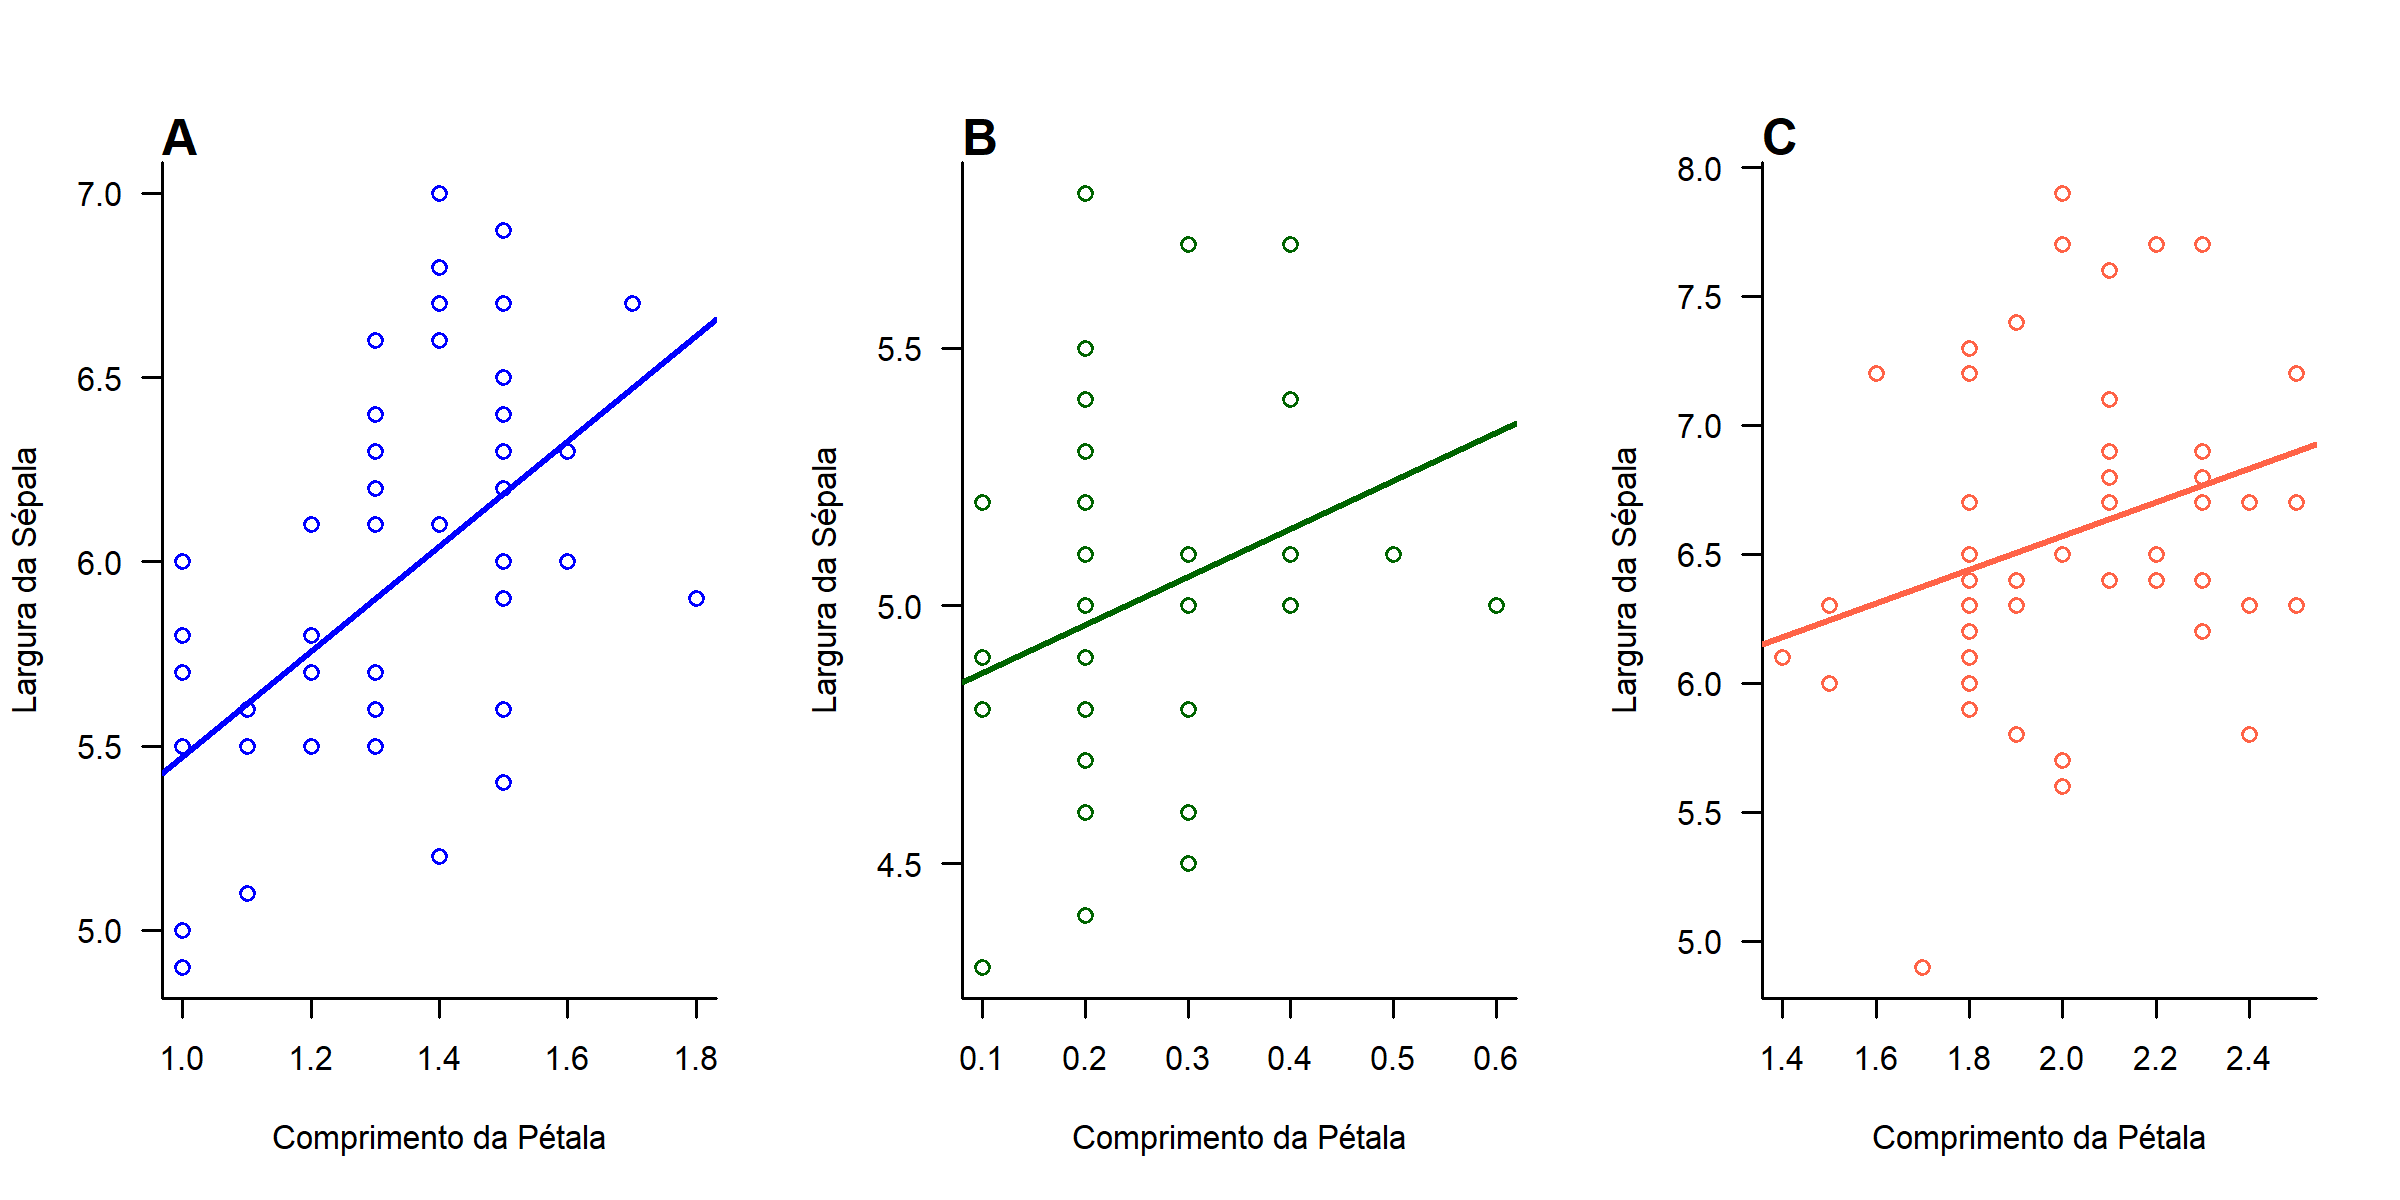
\includegraphics[width=1\linewidth]{../figs/figura04}

Por fim, teremos que exportar este gráfico com as seguintes função:

\begin{Shaded}
\begin{Highlighting}[]
\KeywordTok{png}\NormalTok{(}\StringTok{"figs/figura04.png"}\NormalTok{, }\DataTypeTok{res=}\DecValTok{300}\NormalTok{, }\DataTypeTok{width=}\DecValTok{2400}\NormalTok{, }\DataTypeTok{height=}\DecValTok{1200}\NormalTok{) }\CommentTok{#Essa função deverá ser feita ao início de todo processo de produção do gráfico, pois irá possibilitar uma imagem com os comandos escritos posteriormente. Nesta função teremos que ditar o caminho do arquivo, a resolução em dpi (res=), comprimento (width=), altura (height=).}

\CommentTok{#Ao final de todas as funções para produzir os gráficos, devemos utilizar essa função para salvar em formato de png:}
\KeywordTok{dev.off}\NormalTok{()}
\end{Highlighting}
\end{Shaded}

\begin{verbatim}
## pdf 
##   2
\end{verbatim}


\end{document}
